% Generated by Listas/make_statements.py from pratica-lecture-08.md, item 9. Do not edit.
\textbf{Source.} Gibbons (1992), \emph{Game Theory for Applied Economists}, §4.1 Problems, Problem 4.2, pp.~245--246 {[}PDF pp.~251--252{]}. Reproduced verbatim. Answer: none in the book.



\begin{quote}

4.2. Show that there does not exist a pure-strategy perfect Bayesian equilibrium in the following extensive-form game. What is the mixed-strategy perfect Bayesian equilibrium?



\pandocbounded{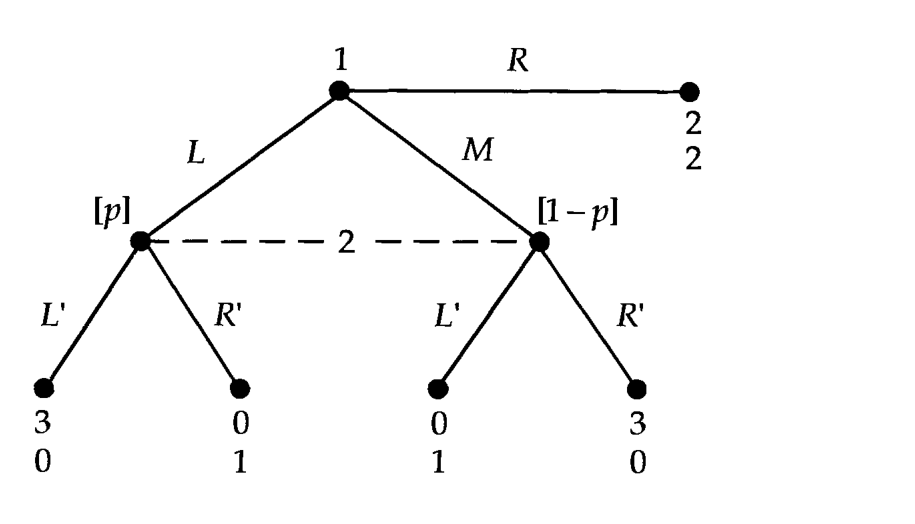
\includegraphics[keepaspectratio,alt={Problem 4.2 extensive-form game}]{../figures/gibbons-4-2.png}}

\end{quote}

